Embedded software often operates in environments critical to human life
and subject to our direct expectations.  We assume that a handheld MP3 
player will perform reliably, or that the unseen aircraft control system
aboard our flight will function safely and correctly.  Embedded environments
require far more care than provided by the current best practices in software
development.  Often formal verification and system certification are required
to insure correct behavior and conformance to legal standards.  Embedded systems
design challenges are well-documented \cite{HenSif:2006}, but industrial 
practice still falls short of these expectations.

Consider one style of modern development practice: graphical modeling and
simulation tools (e.g. Mathworks' Simulink/Stateflow or National Instruments'
Matrix-X) represent physical systems and engineering designs using block 
diagram notations for dataflows or state models.  Design work revolves 
around simulation and test cases, with code generation following once the
design is considered complete.  Such methods frequently ignore software engineering
constraints on the design and neglect issues that arise from embedded 
platform choices.  At early stages of the design, often the platform 
is vaguely specified to the engineers as a set of possible tradeoffs, with
incomplete details regarding actual platform function and performance.

Similarly, another development style uses UML (or similar) tools to capture
software engineering concepts such as components, interactions, timing,
fault handling, and deployment.  These workflows focus on source code 
creation and management followed by testing and debugging on target hardware.
In this case the physical and environmental constraints are not represented
by the tools.  At best such constraints may be provided informally as notes or
documentation to developers and may remain poorly understood.

The interplay between these two prevalent development styles creates
problems.  Designers lack tools to model the interactions between the
hardware, software, and the environment.  For example, software 
generated from a carefully simulated functional dataflow model may 
fail to perform correctly when its functions are distributed over a 
shared network of processing nodes.  Neither style of development 
supports comprehensive verification of certification requirements.  To
move towards a solution to these problems, we propose a suite of tools
that address many of these challenges.  Currently under development at
Vanderbilt's Institute for Software Integrated Systems (ISIS), these 
tools use domain-specific modeling languages (DSMLs) to integrate the disparate
aspects of an embedded systems design.

\begin{figure}[h]
   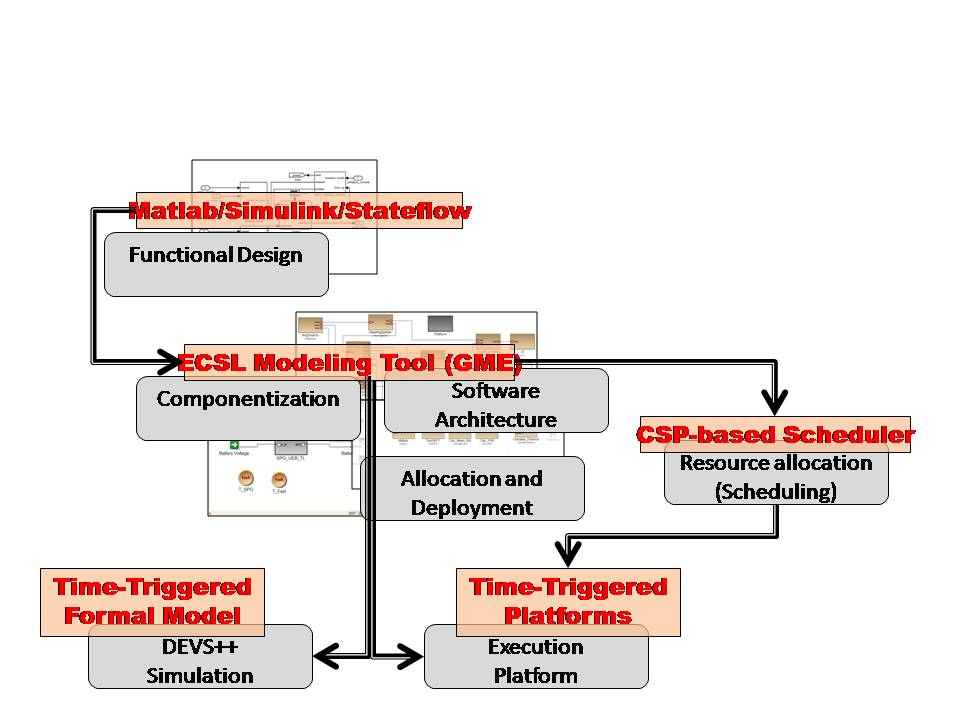
\includegraphics[width=0.9\columnwidth]{existing}
   \caption{Existing elements of the tool suite.}
   \label{fig:existing}
\end{figure}

The tool suite described here is built on the concept of platform-based
design \cite{alberto:2002}, and is shown conceptually in Figure \ref{fig:existing}.  
Componentization and higher-level services enable the designer to build 
correct systems from validated components.  Additionally, if the DSMLs used in 
tool integration have formally defined behavioral semantics and well-defined 
models of computation (MoCs) for component interactions \cite{Lee:M97/11}, system 
properties and models can be expressed formally and verified with appropriate 
external tools.  In the sequel we briefly describe the current state of the tool 
suite and conclude with a discussion of the direction of our future goals.

